%%%%%%%%%%%%%%%%%%%%%%%%%%%%%% -*- Mode: Latex -*- %%%%%%%%%%%%%%%%%%%%%%%%%%%%
%% project.tex -- 
%% Author          : Philip Johnson
%% Created On      : Tue Mar 31 11:44:58 2009
%% Last Modified By: Philip Johnson
%% Last Modified On: Thu Apr 16 15:11:36 2009
%% RCS: $Id$
%%%%%%%%%%%%%%%%%%%%%%%%%%%%%%%%%%%%%%%%%%%%%%%%%%%%%%%%%%%%%%%%%%%%%%%%%%%%%%%
%%   Copyright (C) 2009 
%%%%%%%%%%%%%%%%%%%%%%%%%%%%%%%%%%%%%%%%%%%%%%%%%%%%%%%%%%%%%%%%%%%%%%%%%%%%%%%
%% 

\pagenumbering{arabic}
\renewcommand{\thepage} {C--\arabic{page}}

\renewcommand{\thesection} {C.\arabic{section}}
\setcounter{section}{0}

\section{Project Description}

\subsection{Project Vision, Goals, Objectives, and Outcomes}


{\em Describe the CT-centric vision, goals, objectives, and anticipated
outcomes of the proposed project. Clearly indicate how they will contribute
to realization of the three CPATH program goals: (1) contribute to the
development of a globally competitive U.S. workforce with CT competencies
essential to U.S. leadership in the global innovation enterprise; (2)
increase the number of students developing CT competencies by infusing CT
learning opportunities into undergraduate education in the core computing -
computer and information science and engineering - disciplines, and in
other fields of study; and, (3) demonstrate transformative CT-focused
undergraduate education models that are replicable across a variety of
institutions.  }

\bigskip

Jeannette Wing has written, ``Computational thinking involves solving
problems, designing systems, and understanding human behavior, by drawing
on the concepts fundamental to computer science'' \citep{Wing06}.  In her
presentation ``Computational Thinking and Thinking About Computation'',
Wing refines her view of these fundamental computer science concepts in terms of 
the ``Two As'': Abstraction and Automation.  Activities
related to the first ``A'' include: choosing the right abstractions, operating
at multiple levels of abstraction, and defining relationships between
abstractions.  Activities related to the second ``A'' involve mechanizing the
first A via precise notations and models.  In essence, automation amplifies
the power of abstraction.  Computational thinking, from this perspective,
involves the correct choice of abstraction combined with the correct choice
of automation.

The vision of this proposal is to develop and institutionalize a new
approach to computational thinking where abstraction and automation combine
to transform the use of {\em empirical thinking} in software development.
We call this approach ``empirical computational thinking'', or \eCT.

To introduce our approach, we must first address what is meant by
empirical thinking.  The term ``empirical'' is variously defined as
``derived from experiment and observation rather than theory''; ``evidence
or consequences observable by the senses''; and ``capable of being verified
or disproved by observation or experiment.''

Given these definitions, it is clear that some degree of empirical thinking
is already commonplace in software development.  For example, beginning
programmers use empirical thinking when they ``observe'' the output of the
compiler to learn how to write syntactically correct programs.  Beginners
also tend to make extensive use of ``experimentation'': they execute their
program with example data, compare the actual behavior to what they expect,
then make modifications until the observed behavior matches their
expectations.

These examples of empirical thinking, while typical for beginning
programmers, do not scale well because they lack both abstraction and
automation. Thus, they fail to constitute the kind of computational
thinking of interest to the CPATH program, and they fail as well to be
\eCT.

One would hope that as students progress into more advanced software
development courses, the curriculum would scale in at least two
ways. First, the complexity, size, and number of people involved in a
software development project would scale upwards.  Second, the level of
abstraction and automation in their empirical thinking would scale
commensurately. Unfortunately, while advanced software development courses
certainly require students to develop significantly more sophisticated
systems than their introductory counterparts, the use of empirical thinking
remains mostly non-abstract and non-automated.  The principle computational
support for advanced programming classes is an integrated development
environment such as Eclipse or Visual Studio. While this is a significant
advance over vanilla text editors, such IDEs provide relatively little in
the way of abstraction or automation for empirical thinking about the
products and processes of software development.

Supporting abstraction in empirical thinking for software development
generally means creating quantitative models for important development
concepts.  For example, test quality is an important concept that is
commonly emphasized in advanced software development courses.  One
quantitative model for test quality is line-level test coverage, which is
generally expressed as the percentage of source lines of code in the
software exercised by the test cases.  Another important concept is
complexity, and quantitative models such as afferent and efferent coupling
or cyclomatic complexity provide abstract, empirical representations for
this concept.  Even ``agile'' concepts such as ``commit early, commit
often'' or ``collective code ownership'' can support abstract, empirical
models. For example, ``commit early'' can be modeled as the percentage of
files in the system that are committed within a certain number of days of
their creation.  ``Collective code ownership'' can be modeled by the
percentage of files in the system that have been edited by every member of
the development team.

Supporting automation for these abstractions of empirical thinking for
software development means tool support for collecting, analyzing,
disseminating, and interpreting these abstractions.  For example, an
automated process can run once a day and calculate the current coverage and
complexity values for the system.  These values can be made available to
the user by a web application. Alternatively, email ``alerts'' can be sent
to the developers when coverage crosses a threshold and becomes too low, or
coupling crosses a threshold and becomes too high.  Plugins to development
tools like IDEs can collect information on what files are edited when in
order to determine the age of a file when it is first committed, or the
degree of collective editing on the file.  

Thus, our vision for \eCT includes programming as an activity that is rich
in automated, abstract representations of development processes and
products, made available conveniently and appropriately for observation and
reflection by the programmers.  It also includes education in the analytic
capabilities required to effectively interpret these representations, to
understand their limitations as representations of reality, to know when to
take action based upon them and what kind of action is warranted.

The goal of this research is to explore, evaluate, and institutionalize
techniques and technologies for \eCT, building upon research and education
we have worked on over the past ten years in empirically-based software
engineering.  For example, we recently performed an initial evaluation of a
novel system and associated curriculum we developed called the ``Software
Intensive Care Unit'' \citep{csdl2-09-02}.  In this approach, sensors
attached to development tools automatically collect student process and
product data and abstract it into a set of ten ``vital signs'' that provide
an empirical basis for students to assess the ``health'' of their ongoing
projects.  The Software ICU is an example of \eCT, as it supports both
automated and abstract empirical thinking about the current state and past
history of both their projects and their group processes.  Our curriculum
materials taught students how to introduce the Software ICU data collection
sensors into their laptop development environments, how to obtain the
analyses, and how to interpret the results.

While we are excited by the potential of our own prior work in \eCT, there
are other research and educational initiatives that conform to our broader
vision for \eCT.  Our goal is to organize and develop a constellation of
approaches to \eCT and build a body of knowledge that enables future
researchers and educators to understand the comparative strengths and
weaknesses of the various approaches and to create innovative new
approaches to \eCT that go synthesize and/or extend beyond any of the
present day capabilities.

To achieve this goal, we will pursue three concrete objectives, organized
according to the three years of this grant.  

First, we will perform a study during the 2009-2010 academic year at the
University of Hawaii in which we will validate and extend the findings from
our initial case study of the Software ICU during 2008.  We will also begin
trial use of a second approach to \eCT we have developed called Devcathlon. 
Finally, we will begin development of a common evaluation framework for \eCT that
can be used to 

Second, we will partner with other academic institutions and departments
during the 2010-2011 academic year to gain insight into the issues that
occur when integrating empirical thinking into other advanced software
development courses.  In addition, we will begin exploring the issues
involved in adapting these initial materials both downward (into more
elementary curriculum); upward (into post-scholastic, professsional
settings); and outward (into related disciplines such as engineering or
information technology).

Third, we will use the data gathered and the collaborations formed during
the first two years to form an open source consortium to further spread the
use of abstract, automated empirical thinking.  This consortium will itself
be transformative in that it will combine open source technologies (such as
the Software ICU and Devcathlon) with open source curriculum materials
(which facilitate the introduction of the materials) with open source data
(results from the application of these technologies and pedagogies, which
can be used to guide future evolution of these approach).  The goal is to
go far beyond web site publication and create a social network of students
and educators interested in advancing the use of empirical thinking in
software development

Our vision, goal, and objectives are designed to produce outcomes that
directly support the goals of the CPATH program.  First, establishing
automated, abstract empirical thinking as an integral component of software
development courses can significantly improve the competitiveness of our
software engineering workforce by giving them facility with a powerful tool
for computational thinking.  Second, our approach begins by infusing a new,
empirical form of computational thinking into the advanced software
development curriculum and then propogates it downward, upward, and
outward.  Third, we will collect data and experiences on the effectiveness
of this approach across a variety of institutions and pedagogical models.

\subsection{Intellectual Basis/Related Work}

{\em Describe the intellectual basis for the project and discuss related
prior work.  Include a review of the research literature relevant to the
project and provide corresponding references. }

\bigskip

\subsubsection{Research from the empirical software engineering community}

As noted above, empirical thinking occurs naturally in software development
activities.  There is a well-established research community focusing on the
promulgation and advancement of empirical techniques in software
development.  Organizations such as the International Software Engineering
Research Network (ISERN), journals such as Empirical Software Engineering,
and conferences such as the International Symposium on Empirical Software
Engineering and Measurement all provide active forums for the role of
empirical thinking in software development.

Unfortunately, review of these forums indicates that the role of empirical
thinking in the software development curriculum receives relatively little
attention.  For example, in the 328 articles published in Empirical
Software Engineering from 2002 to 2008, we found only one article that
focused explicitly on the use of empirical techniques as part of software
development pedagogy \citep{Pfahl03}.  Through review of the other
articles, we found that while students are frequently employed in empirical
research, the goal of their participation is to support the testing of a
research hypothesis unrelated to classroom pedagogy.  For example,
\cite{Babar08} used students to support a controlled study of the
differences between distributed and face-to-face meetings for software
architecture evaluation.  \cite{Carver06} used students as subjects to test
an approach for helping novice programmers learn software inspection
techniques more quickly.  \cite{Host00} performed a study in which students
were used to determine if the data collected from students differs from
data collected from professionals.

The Dagstuhl Workshop on Empirical Software Engineering Issues
\citep{Basili06} contained a track on educational issues, but a primary
focus was the use of students as subjects for empirical experimentation.

The Empirical Studies of Programmers workshop series (now discontinued)
focused on the use of empirical technique to understand programmer
behavior, rather than teaching students how to use empirical thinking to
affect their own behavior.  This emphasis is shared to a great extent by
the Journal of Educational Resources in Computing, now renamed ACM
Transactions on Computing Education.

The Empirical Software Engineering and Measurement conference series has
provided a forum for a variety of applications of empirical techniques,
including those for testing and analysis, coordination and communication,
estimation, modeling and architecture, inspections, defect classification,
and fault-prone module prediction.  We found only one paper that focused
explicitly on the introduction of empirical techniques into the classroom
setting was \citep{csdl2-03-12}.

Finally, we have directly solicited information about their classroom
pedagocy from the empirical software engineering community using internal
mailing lists and personal contacts. We found evidence that courses at a
variety of universities include material related to empirical techniques,
including: University of Rome/Tor Vergata; Mississippi State University;
Norwegian University of Science and Technology; University of Insubria;
University of Southern California; University of Maryland; University of
Bari; University of Sheffield; Seattle University; University of Virginia;
University of Ottawa; Keele University; University of Karlsruhe;
Polytechnical University of Madrid; University of Calgary; and University
of Toronto.  However, the material was generally related to using students
as subjects (undergraduate level) or the teaching of experimental
methodologies (graduate level).  One exception is the University of
Southern California, where students gather empirical data for abstraction
using the COCOMO cost modeling system to estimate effort and time for their
projects.

\subsubsection{Research in the software engineering education community}

The previous section demonstrates that the empirical software engineering
community does not (yet) focus on the pedagogy of empirical thinking. Fortunately, 
there is more evidence of interest in this approach in the software education 
research community.

In 1995, Watts Humphrey authored {\em A Discipline for Software
Engineering}, a ground-breaking text that adapted organizational-level
software measurement and analysis techniques to the individual developer
along with a one semester curriculum. These techniques are called the
Personal Software Process (PSP), and form the basis for the Team Software
Process (TSP), which extends the method to groups of developers. 

The PSP is the best known and most widespread approach to empirical
thinking in the advanced software development curriculum.  The approach
requires students to develop a series of software projects, typically six
to eight during a single semester.  Both process and product measures are
gathered about each project, and the measurements become increasingly
detailed as the semester proceeds. After the first three projects are
completed, the students can use the completed projects as historical data
to support quality improvement (by identifying repeated types of defects)
and estimation (through simple linear regression).  The PSP and TSP enjoy
strong support from the Software Engineering Institute, which has published
a number of case studies indicating success in a classroom setting and
which sponsors a yearly symposium to publicize academic and industry
experiences.  The PSP/TSP enable support for very basic levels of
abstraction and automation of empirical thinking. For example, the PSP
Dashboard is a tool that allows students to enter the data they collect and
which will automate the calculation of regression lines.

Conn developed a metrics-based software engineering course called the 
IS Integrated Capstone Project \cite{Conn04}.  The metrics were closely aligned
with the PSP/TSP format, though some of the process constraints were relaxed. 

Robillard designed a project-based course in which students were required
to fill out logs that specified the time spent on various activities
\cite{Robillard98}.  However, minimal abstraction and no automation was supported.

One recent research effort shows how abstract and automated empirical
thinking can be used in introductory programming courses. The Retina system
automatically collects editing and compilation data on beginning
programmers, which it then abstracts using a recommendation and suggestion
subsystem \cite{Murphy09}.  Retina can notice, for example, when a student
is getting many more errors per compilation than other students in the
class, and recommend that the student might want to break the work down
into smaller pieces.  Retina is designed around the needs of introductory
programming classes, where students typically work alone, do not use a wide
range of development tools, and a significant amount of energy is devoted
to obtaining a syntactically correct program.  Nevertheless, it
demonstrates that there is significant potential for the use of abstract,
automated, empirical thinking throughout the software development
curriculum.

\subsubsection{From empirical to scientific and evidence-based thinking}

Integrating computational thinking concepts (automation and abstraction)
with empirical thinking has the potential to transform and improve the
software development curriculum in profound ways. One of the most important
benefits of introducing empirical thinking is that it is a necessary
precursor for scientific and evidence-based thinking in software
development.

One of the most eloquent descriptions of the difference between empirical
and scientific thinking is provided by John Dewey \citep{Dewey10}.  In his
chapter ``Empirical and Scientific Thinking'', Dewey begins by noting that
empirical thinking, which is based purely on observation, has been used by
humans throughout history as a way of understanding through association.
For example, upon repeatedly noticing that when the sky is lowering upon
sunset, rain follows the next day, one might form the ``conclusion'' that
if the sky is lowering at sunset, rain will follow.  He follows this with a
discussion of the danger of confusing correlation with causality, and
introduces the scientific method as a way of addressing this problem.  From
Dewey's point of view, the scientific method involves active
experimentation under controlled or semi-controlled conditions (as opposed
to passive observation) and the formation of testable theories that
introduce causal mechanisms (for which evidence can be gathered to support,
refute, or refine).  A major focus of the empirical software engineering
community is to develop experimental techniques applicable to software
development practice that replace simple observation with more controlled,
hypothesis-driven analysis.

A related effort is the application of evidence-based medical research
techniques to software development \citep{Kitchenham04,Kitchenham04a},
which involves a five step method: (1) Convert the need for information
[about a software engineering practice] into an answerable question; (2)
Track down the best evidence available for answering the question; (3)
Critically appraise that evidence using systematic review for its validity
(closeness to the truth), impact (size of the effect), and applicability
(usefulness in software development practice); (4) Integrate the critical
appraisal with current software engineering knowledge and stakeholder
values [to support decision-making]; (5) Evaluate the effectiveness and
efficiency in applying Steps 1-4 and seek ways to improve them for next
time.  While promising, application of systematic reviews and the
integration of empirical software engineering data from multiple sources
has been found to be challenging \citep{Jedlitschka04}.  Evidence-based
software engineering is also a topic of interest to the empirical software
engineering community.

%% GQM??

\subsubsection{Conclusions}

From review of this related work, we can see that the empirical software
development method with the longest history and most industrial support is
the PSP/TSP.  However, it enjoys relatively limited levels of abstraction
and automation.  It is also purely observational in nature and does not
integrate scientific or evidence-based methods.

We can also see that there is a tremendous opportunity for synergy with the
empirical software engineering community by collaborating on development of
curriculum that engages students as direct participants in empirical
observation and analysis.  The University of Southern California has
demonstrated that this is possible.

There is also evidence that abstract and automated empirical thinking can
be applied outside the confines of advanced software development courses.
The Retina system shows how even introductory courses can benefit.


\subsection{Current State}

{\em Provide a current assessment of undergraduate education in the
relevant participating organizations.  Describe prior pilot programs or
planning activities conducted to date, if any, and their outcomes.  Where
appropriate, provide institutional data to document the current environment
by uploading data into the Supplementary Docs section in FastLane.}

\bigskip

For over ten years, we have been exploring empirical software engineering
techniques and their applications in the classroom setting as part of our
research in the Collaborative Software Development Laboratory at the
University of Hawaii.  This section summarizes our prior studies and the
current state of practice in our institution.

{\bf PSP.} Beginning in the late 1990's, we instituted the use
of the Personal Software Process in both undergraduate and graduate
software engineering courses.  While our outcomes were quite positive and
in line with the data gathered by the Software Engineering Institute, we
were concerned by the possibility of data quality problems and the lack of
automation.  To investigate the first question, we undertook a study of PSP
data quality which found that manual collection and analysis could result
in data quality problems that could effect the outcomes and interpretation
of the data \citep{csdl-98-13,csdl-98-11}.  To investigate the second question, we
implemented extensive tool support for PSP/TSP style of data collection and
analysis \citep{csdl2-00-03}, but still found the overhead to be
substantial\citep{csdl2-01-12}. 

{\bf Hackystat.} In 2001, we initiated a research project called Hackystat
\citep{csdl2-06-06,csdl2-04-11,csdl2-02-07}, one of whose goals is to
support abstract and automated empirical thinking in the classroom setting
in a manner different from the PSP/TSP.  To accomplish this, we changed the
types of data collected and the nature of the analyses and interpretations
provided by the framework.  For example, in the PSP/TSP (as well as other
approaches like COCOMO), data on completed projects is used to make
predictions about future, as-yet-unstarted projects. Hackystat
instead uses ``sensors'' attached to development tools to automatically and
unobtrusively collect fine-grained process and product data. Analyses on
this data are intended for direct feedback into the current system under
development, not for use in future system planning.

For the past five years, Hackystat has been an integral part of the
University of Hawaii software engineering curriculum at both the
undergraduate and graduate levels.  We performed case study experiments in
2003 \citep{csdl2-03-12,csdl2-03-13}, 2006 \citep{csdl2-07-02}, and 2008
\citep{csdl2-09-02,csdl2-09-03} to assess the classroom impact and
effectiveness of the system in supported automated and abstract empirical
thinking.  Each case study collected both quantitative and qualitative data
that motivated extensive redesign and improvement of the system, which we
evaluated in the subsequent case study. While the details of evaluation
differed in the three studies, in all cases we were generally concerned
with three issues: (1) What was the perceived overhead of the system? In
other words, how well does the system provide automation?  (2) What was the
perceived utility of the system? In other words, how well does the system
provide abstraction?  (3) How well will the system apply to
``professional'' settings?  In other words, to what extent does the
empirical thinking promoted by this system feel relevant and useful in the
long term?

These case studies generated a great deal of useful data that has directly
influenced the course of our research and educational practice. For
example, the 2003 experiment provided data indicating that sensor
installation was perceived as a significant barrier to use. From the \eCT
perspective, this is an example of a failure of the system to provide
sufficient automation.  The 2006 experiment provided data indicating that
students had difficulties interpreting the trends in data and understanding
when the data indicated the need for a change in behavior.  From the \eCT
perspective, this is an example of a failure of the system to provide
sufficient abstraction.  In all three case studies, students have raised
concerns about privacy issues.  This is an example of a challenge and
potential limitation of this approach to support empirical thinking.

{\bf Software ICU.}  In 2008, we performed an initial case study evaluation 
of a new approach to teaching \eCT concepts.  In this approach, we frame 
\eCT within the metaphor of a medical intensive care unit (ICU). 

Medical intensive care units feature automatic and continuous monitoring of
patient vital signs.  The four fundamental medical vital signs are
temperature, heart rate, blood pressure and respiration.  Other vital signs
may be monitored depending upon the particulars of a patient condition.
Vital signs have a ``normal range of behavior'', and the monitoring unit
can raise an alarm when any of the patient's vital signs departs from its
normal range of behavior.

Vital signs are interesting because: (a) in a healthy patient, they are
normal or improving; (b) change in one vital sign may or may not be
significant; (c) change in multiple vital signs is almost certainly
significant, particularly if more than one are outside their normal range.

The Software ICU translates ``health'', ``ital signs'', ``normal range''
and the ICU monitoring user interface into terms useful to students and their
software development projects.

We defined a healthy development project as satisfying three high-level
characteristics: high efficiency (software development proceeds ``as fast
as possible, but no faster''); high effectiveness (effort is focused on the
most important issues, with minimal rework); and high quality (software
satisfies user needs; software can be easily installed, adapted, and
maintained).

We then presented a set of simple practices that, if followed, we claimed
would improve the health of their projects.  These included: everyone works
consistently; everyone contributes equally; code is committed consistently;
progress is regular; quality remains high; no last minute rush to finish.
These development practices are analogous to life-style behaviors like
``eat right'', ``get enough sleep'' and ``exercise regularly'' that
generally facilitate (but, of course, do not guarantee) good health in a
patient.

Next, we presented nine software vital signs: coverage, complexity,
coupling, churn, builds, commits, unit tests, size, and dev time. Through a
combination of Hackystat sensors and the Hudson continuous integration
system, these nine vital signs could be automatically and continuously
collected for their projects.

For each software vital sign, we then presented its normal range of
behavior.  For example, for the coupling vital sign to be considered
healthy, its current value should be above 90\% and the trend in
coverage over time should be stable or increasing.  For the commit vital
sign to be considered normal, at least 50\% of the team members should have
committed, and there should be commits on at least 50\% of the days in the
project interval.  For one of the vital signs, size, we stated that
there is no simple way of assessing its normal range of behavior, though
it still provides some value in understanding project health.

Unlike a medical ICU, where there is literally hundreds of years of medical
research establishing both the importance of the four fundamental vital
signs and their normal range of behaviors, no such consensus exists in
software engineering on what would constitute ``fundamental'' software
vital signs or their normal range of behavior.  Thus, our selection of
software vital signs and their normal range of behaviors are actually
research hypotheses.  We designed a case study to elicit evidence
regarding the appropriateness of these vital signs and our proposed normal
range of behaviors.

Finally, we presented the user interface to the Software ICU. A portion of
this user interface appears in Figure \ref{fig:sicu}.

\begin{figure*}[ht]
  \center
  \includegraphics[width=0.8\textwidth]{portfolio-2008.eps}
  \caption{An example Software ICU display}
  \label{fig:sicu}
\end{figure*} 

Each row in the Software ICU interface provides information about one
software project.  Each column presents information about one vital
sign. Similar to the medical ICU, the software ICU presents both the most
recent numeric value as well as the recent trend in value for each vital
sign.  The normal range of behavior is represented by independently
coloring the trend line and the most recent value as green, yellow, or red
depending upon whether the value was healthy, unstable, or unhealthy.

The measurements underlying the Software ICU were collected automatically
through two mechanisms. First, the students installed Hackystat sensors
into their IDE (Eclipse) and build system (Ant) which sent process
metrics regarding their development activities.  Second, their projects
used the Hudson system to perform continuous integration, which meant that
after each commit of their code, the system would be automatically built
and tested.  The Hudson system was also configured to automatically gather
certain product metrics such as coverage, coupling, and complexity.

{\bf Devcathlon.} A current active research and development project involves
the creation of an environment in which \eCT principles are embedded within
a game environment.  Unlike other software development games which rely on
simulation of developer activities \cite{simSE}, Devcathlon is designed
around the use of actual data collected from students as they develop
software.  Students can form teams and play matches against each other.
Matches are based upon ``events'' which reward teams for appropriate
software development behaviors, such as ``commit early, commit often'',
``keep the coverage high'', and ``don't break the build''.

As of Spring, 2009, Devcathlon is under active development and we expect to
have an initial release for evaluation by Fall of 2009.


\subsection{Implementation Plan}

{\em Describe in detail the CT-centric activities to be undertaken to
realize the project vision, goals, objectives and anticipated outcomes.

Define, or describe how the proposing team will attempt to define, the core
computing concepts, methods, technologies and tools to be integrated into
promising new undergraduate education models.  Describe your plans to
identify and implement effective strategies to develop and assess CT
competencies in the relevant learning communities.  Identify the
stakeholder cohort, e.g. K-20 administrators, faculty, teachers, students,
etc., that will participate in and/or benefit from the activities. If
relevant, describe how change will be effected and sustained in the
participating organizations.

Describe project milestones in the context of a project timeline and
identify responsible parties and expected outcomes for each milestone.
Summarize this information in a figure that you upload into the
Supplementary Docs section in FastLane.

Describe how project outputs and outcomes will be disseminated to the
relevant stakeholder groups and to the national community and if relevant,
how project resources will be made available to others to adopt or
adapt. Identify proactive measures to find and support adopters of
promising models and/or practices. Describe plans for outreach to other
groups or interested institutions that will take place during the project.
}

Our implementation plan is comprised of several functional activities to be distributed across the three years of the project.

{\bf Common \eCT Evaluation Framework development.}  A primary objective of
this project is to develop a framework for evaluation of \eCT curriculum
materials.  The goal of this evaluation framework is to elicit useful
information concerning the ways in which the particular approach to \eCT
provides for empirical, automated, and abstract thinking. Some examples of
the data to be collected include: (a) the targeted population of students
for which this approach is geared; (b) the specific kinds of observations
gathered; (c) the specific abstractions made available and their
inter-relationships; (d) the specific forms of automation provided; (e) the
forms of student feedback about the system; (f) mechanisms for post-course
follow-up to see the downstream effect of the \eCT experience.

The development of the Common \eCT Evaluation Framework will be ongoing
throughout the project.  During the first year of the project,
framework-related activities will consist of simply collecting information
about the ways in which various \eCT efforts address these issues. We
expect there to be wide diversity in the way different groups approach
these issues. This first year of data gathering will form our ``baseline''.
In subsequent years, we will use this baseline data to help push the \eCT
community in two directions. First, the baseline should help the community
move forward toward more consistent, higher quality evaluation
mechanisms. For example, if one group has developed a particularly good
instrument for assessing student opinion, then the baseline can make this
apparent and help spread its use to other organizations.  Second, the
baseline can identify opportunities for synergy.  For example, it might
surface separate approaches to \eCT that could be synergistically combined.

To help make this idea concrete, Figure
\ref{fig:cef} provides a cursory overview of four \eCT curriculum efforts. 

\begin{figure}[th]
\small
\begin{tabular}{|p{0.50in}|p{1.25in}|p{1.25in}|p{1.25in}|p{1.25in}|} \hline
{\bf \eCT} & {\bf Population} & {\bf Observations} & {\bf Automation} & {\bf Abstraction} \\ \hline

Software ICU & 
Advanced  &
Development tool use, analysis output & 
Plugins to Development tools &
Coverage, DevTime, Coupling, (others) \\ \hline

Retina &
Beginning  &
Compilation events &
Plugins to Eclipse &
Behavioral recommendations \\ \hline

PSP/TSP &
Advanced &
Size, time, defects &
Regression analysis &
Effort/quality prediction \\ \hline

SimSE &
Advanced &
employees, artifacts, customers &
simulated development &
process models, project success \\ \hline

\end{tabular} 
\caption{Sample \eCT approaches}
\label{fig:cef}
\normalsize
\end{figure}

The Common \eCT Framework will collect much more detailed information about
\eCT efforts than Figure \ref{fig:cef}, but the Figure does illuminate
aspects of the framework.  First, the framework will not typically provide
information that enables a researcher or practitioner to conclude that one
\eCT approach is ``better'' than another.  The goals and approaches are
much too diverse for that.  Rather, the framework will be designed to
illuminate opportunities for synergy. For example, the PSP/TSP provides
data useful for pre-project planning, while the Software ICU provides data
useful for in-project course correction.  Thus, these two approaches target
different aspects of software development and suggests an opportunity for a
combined, hybrid approach.  Another example of synergy is the
recommendation engine in Retina: could that technology be adapted for use
with advanced, rather than introductory students? Another opportunity not
illustrated in Figure \ref{fig:cef} concerns evaluation.  While the
Software ICU and Retina have only been evaluated in one university setting
\cite{softicu,retina}, both SimSE and the PSP/TSP have been evaluated in
multiple university settings \cite{simse-multi,psp-multi}.  Comparison of
these approaches can provide insights of use to future multi-site
evaluation for those approaches that have not yet been evaluated in that
way.

{\bf \eCT curriculum development.}  A second functional area involves
enhancement of our current \eCT curriculum involving the Software ICU and
Devcathlon. We plan to use and evaluate both of these approaches in the
software engineering curriculum at the University of Hawaii over the course
of the project.  Feedback from our initial case study \cite{softwareicu}
has surfaced a variety of opportunities for improvement in the Software
ICU, and we have yet to deploy Devcathlon in a classroom setting.

While our prior experience provides a rich set of enhancements to these
systems, we look forward to the results of the first year of the project,
when the baseline data from the \eCT Common Evaluation Framework becomes
available.  This will generate a second source of improvement opportunities
for both the Software ICU and Devcathlon, based upon analysis of the
strengths, weaknesses, and application of other \eCT technologies.

{\bf \eCT curriculum dissemination.}  





\subsection{Collaboration and Management Plan}

{\em Provide a collaboration and management plan that will guide project implementation.  Describe how the project leadership team will form, orient, manage, and reinforce relationships in the project.  Provide evidence of the commitment of the participating organizations to effect and sustain the anticipated project outcomes; letters of collaborative support should be uploaded into the Supplementary Docs section in FastLane. }

Unify the PSP and Hackystat approaches. also PROM etc. Jazz. 

Create an internationally-based consortiium

\subsection{Evaluation Plan}

{\em Provide an evaluation plan that will inform the project progress and measure its impact.  Include a description of the instruments/metrics used to measure, document, and report on the project's progress.  Identify the evaluator who will be responsible for the evaluation component and discuss their expertise related to the evaluation as well as any other linkages to the project or organizations involved.  }



%% Letters of support
%%  Referentia
%%  Blanca Polo (community college level) blanca@hawaii.edu
%%  Gail Kaiser kaiser@cs.columbia.edu
%%  Vic Basili/UMD.  Special issue? basili@fc-md.umd.edu
%%  Lionel Briand? briand@sce.carleton.ca
%%  Pekka   	 Pekka.Abrahamsson@cs.helsinki.fi
%%  Hakan  Hakan.Erdogmus@nrc-cnrc.gc.ca
%%  Laurie Williams, Open seminar, Eclipse/Jazz williams@csc.ncsu.edu
%%  Barry Boehm
%%  Dan Port (ITM) 
%%  Brian Pentland 
%%  The friend of Brian who visited apache foundation, etc. 
%%  Claes
%%  Morisio
%% Japan? 

%%  Contents of letter: importance of empirical thinking in software engineering; soundness of this research approach; potential interest in collaboration; 


